\documentclass{article}
% translate with >> pdflatex -shell-escape <file>

% This file is an extract of the PGFPLOTS manual, copyright by Christian Feuersaenger.
% 
% Feel free to use it as long as you cite the pgfplots manual properly.
%
% See
%   http://pgfplots.sourceforge.net/pgfplots.pdf
% for the complete manual.
%
% Any required input files (for <plot table> or <plot file> or the table package) can be downloaded
% at
% http://www.ctan.org/tex-archive/graphics/pgf/contrib/pgfplots/doc/latex/
% and
% http://www.ctan.org/tex-archive/graphics/pgf/contrib/pgfplots/doc/latex/plotdata/

\usepackage{pgfplots}
\pgfplotsset{compat=newest}

\pagestyle{empty}

\begin{document}
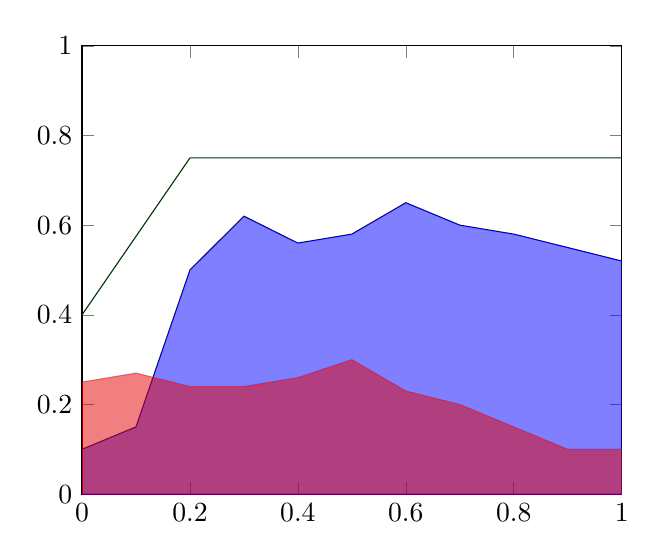
\begin{tikzpicture}
\begin{axis}[ymin=0,ymax=1,enlargelimits=false]
\addplot
	[blue!80!black,fill=blue,fill opacity=0.5] 
coordinates
{(0,0.1)    (0.1,0.15)  (0.2,0.5)   (0.3,0.62)
 (0.4,0.56) (0.5,0.58)  (0.6,0.65)  (0.7,0.6)
 (0.8,0.58) (0.9,0.55)  (1,0.52)} 
|- (axis cs:0,0) -- cycle;

\addplot
	[red,fill=red!90!black,opacity=0.5]
coordinates 
{(0,0.25)   (0.1,0.27)  (0.2,0.24)  (0.3,0.24)
 (0.4,0.26) (0.5,0.3)   (0.6,0.23)  (0.7,0.2)
 (0.8,0.15) (0.9,0.1)   (1,0.1)}
|- (axis cs:0,0) -- cycle;

\addplot[green!20!black] coordinates
	{(0,0.4) (0.2,0.75) (1,0.75)};
\end{axis}
\end{tikzpicture}
\end{document}
